\chapter{Literature Review}

\section{Introduction}

The purpose of this literature review is to synthesise and critically evaluate existing research relevant to the design of an Integrated Data Repository (IDR) and operational analytics dashboard aimed at improving post-MDT oncology pathway efficiency. Timely cancer treatment has profound implications for survival, patient experience, resource utilisation, and system performance. Evidence from national datasets, observational studies, systematic reviews, and informatics research shows that delays between MDT decisions and treatment initiation remain persistent across the NHS. Furthermore, data fragmentation, inconsistent recording practices, and limited visibility of operational bottlenecks hinder the ability of clinicians, MDT coordinators, and service managers to proactively manage these delays.

The review is organised around five interrelated themes:
\begin{enumerate}
    \item MDT operations and evolving pressures on multidisciplinary cancer decision making;
    \item Operational delays across the cancer pathway, particularly diagnosis-to-treatment intervals (DTI);
    \item Data fragmentation and the case for integrated data repositories;
    \item Dashboards and performance-monitoring tools to support operational decision-making;
    \item Emerging data trends and the role of ETL, interoperability, AI and multimodal data integration.
\end{enumerate}

Collectively, this literature forms the conceptual foundation (kernel theory) for the artefact developed in this study. The following sections provide a detailed account of these themes, integrating high-quality evidence from the UK, international datasets, clinical oncology, health informatics, and organisational science.

\subsection{Method}
An iterative literature review was adopted, following the guidance outlined by  \cite{dawson2015} (Figure \ref{fig:LitProc}). An initial search was conducted using Google Scholar and open-access repositories to identify foundational concepts and terminology related to Integrated Data Repositories, cancer pathways, MDT operations, dashboards, and Design Science Research. These preliminary results informed a more structured search strategy applied to ScienceDirect, IEEEXplore, and PubMed.

Searches were limited to peer-reviewed journals, systematic reviews, national audits, and authoritative policy documents published primarily between 2010 and 2026, with earlier seminal works retained where conceptually relevant (e.g. JCCO report \citep{ash2004}, the Calman-Hine report \citep{calman1995} and Design Science Research foundations). Studies were included if they addressed MDT processes, oncology pathway delays, health data integration, dashboards, usability standards, or operational analytics. Articles focused exclusively in molecular biology, single-modality clinical trials, or non-healthcare data systems were excluded. 

Approximately 90 sources were reviewed during the process, with around 55 core studies retained for detailed analysis based on relevance, methodological quality, and applicability to NHS operational contexts. Backward citation tracking was used to identify influential seed papers and ensure conceptual completeness.

\begin{figure}
    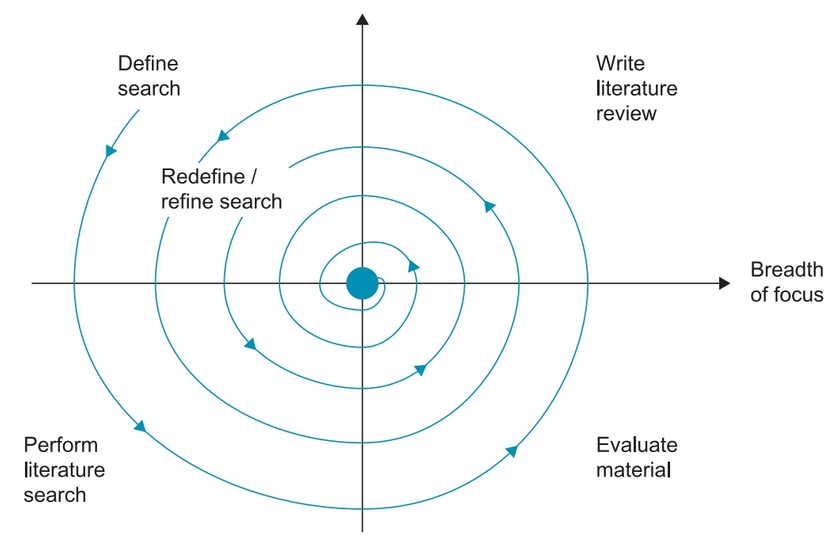
\includegraphics[width=\linewidth]{LitProc.png}
    \caption{Iterative literate review process \citep{dawson2015}}
    \label{fig:LitProc}
\end{figure}

\section{The NHS Cancer Pathway and MDT Framework}

\subsection{MDTs as the Backbone of UK Cancer Care}

Since the publication of the Calman–Hine report \citep{calman1995} and subsequent interventions, MDTs have been embedded as the central governance structure for cancer decision making \citep{haward2006, price2014, morris2006, morris2008}. The MDT model mandates that every new cancer case in the UK is discussed by a multidisciplinary panel including oncologists, surgeons, radiologists, pathologists, specialist nurses, and allied professionals. The 2024 NHS Wales MDT Charter emphasises the crucial role MDTs play in standardising care, reducing unwarranted variation, and improving outcomes by bringing domain experts together in real time \citep{nhswales2024}. Prospective benefits include higher adherence to guidelines, improved communication, shared decision-making, and better coordination of multi-modal treatment plans.

However, the complexity of modern cancer care has increased dramatically alongside rising incidence, new treatment options, biomarker-based stratification, digital imaging volume, and genomic data availability. MDTs now contend with substantially larger case numbers, more complex diagnostic information, and resource pressures that stretch meeting capacity. Professional societies and national audits consistently highlight that MDT meetings are often over-subscribed, under-resourced, and administratively burdensome. These pressures compromise the quality of discussion and create operational bottlenecks that directly affect patient pathways.

\subsection{Evidence of MDT Operational Pressures}

Several studies provide evidence of the challenges affecting MDT functioning:

\begin{itemize}
    \item \cite{soukup2022} conducted a detailed observational analysis of 822 case discussions across three UK MDTs. Administrative and process issues occurred in 30\% of cases, attendance problems in 16\%, and equipment issues in 5\%. These logistical challenges significantly reduced the quality of information and decision-making, demonstrating how operational inefficiencies detract from MDT effectiveness.
    \item \cite{lim2025} analysed 1,488 UK Head and Neck Cancer patients across 50 MDTs and found extremely low compliance with national cancer pathway standards: 32.8\% (FDS), 33.3\% (31‑day), and 34.6\% (62‑day). Median DTT-to-treatment was 42 days.
    \item \cite{chakravarty2023} demonstrated that patients referred from secondary-care outpatient pathways experienced significantly longer delays to MDT discussion and treatment (mean 102 vs. 88 days). These patients were also more likely to receive palliative rather than curative treatment.
    \item \cite{law2024} identified a decade of known MDT barriers including time pressures, communication challenges, inconsistent attendance, information deficits, and increasing clinical complexity.
\end{itemize}

While these studies consistently demonstrate operational strain within MDT processes, several limitations should be acknowledged. Much of the existing evidence is observational and focuses primarily on meeting effectiveness, communication quality, or decision-making processes rather than downstream operational consequences following MDT outcomes.For example, \cite{soukup2022} identify logistical and administrative barriers that impair MDT performance, yet the study does not examine whether these issues translate into measurable delays in treatment initiation. Similarly, the scoping review proposed by \cite{law2024} aggregates a broad range of organisational challenges but provides limited insight into which barriers exert the greatest influence on pathway performance.   

Large-scale cohort studies such as \cite{lim2025} quantify poor compliance with national standards, but their retrospective design offers little visibility of the specific workflow stages responsible for delay accumulation. Consequently, while the literature establishes that MDT processes operate under significant pressure, a gap remains in understanding how operational data can be used to identify, monitor, and mitigate delays arising after MDT decisions have been made. This distinction is important because improving MDT discussion quality alone may be insufficient if subsequent scheduling and treatment processes remain poorly coordinated.

\subsection{National policy direction and waiting time standards}

NHS England's 2024/25 planning guidance emphasises compliance with the Faster Diagnosis Standard (FDS) and cancer treatment timeliness metrics. Persistent waiting-time challenges, data-quality requirements, and the need for integrated pathway oversight tools are highlighted \citep{parker2026}. Radiotherapy services face particular strain: the Royal College of Radiologists reported over 2,300 breaches of the 31‑day standard in October 2023 \citep{rcr2024}. Hidden waits—such as 20‑week delays between surgery and radiotherapy—are not systematically captured, further illustrating limitations in operational visibility.

\section{Operational Delays in Cancer Pathways}

\subsection{Diagnosis-to-Treatment Interval (DTI) as a Critical Metric}

A robust body of literature demonstrates that prolonged DTI adversely affects survival across multiple cancer types.

Key findings include:

\begin{itemize}
    \item \cite{hanna2020}: A systematic review of 34 studies (1.27M patients) found each four-week delay increased mortality by up to 6–8\% across treatment modalities.
    \item \cite{coca-pelaz2018}: Delays in Head and Neck Small Cell Carcinoma beyond four weeks contribute to tumour progression and reduced local control.
    \item \cite{sharma2016}: Delays greater than 30 days reduce overall survival (HR 1.12), with mortality increasing 2.2\% per additional week.
    \item \cite{villemure-poliquin2025}: Treatment within 30 days improves survival by 9\%.
    \item \cite{saleh2024}: Cervical cancer survival drops dramatically after 30 days.
\end{itemize}

\subsection{Hospital/System Factors Influencing Delay}

Large-scale evidence shows that delays are driven not only by tumour characteristics but also by organisational inefficiencies:

\begin{itemize}
    \item \cite{yun2012}: Delays over one month worsened outcomes, especially in low-volume hospitals.
    \item UK audits (e.g., \cite{lim2025}) highlight delays in biopsies, imaging, scheduling, and treatment booking.
\end{itemize}

A further limitation of the current literature is the tendency to treat organisational performance as a static characteristic rather than a dynamic process. Factors such as hospital volume, resource availability, and service configuration are frequently associated with treatment delays; however, there is comparatively little exploration of how these risks evolve over time or how operational teams can intervene before delays become breaches. This reinforces the distinction between retrospective performance measurement and proactive pathway management.

\subsection{MDT-specific drivers of post-decision delays}

\begin{itemize}
    \item Missing diagnostic information and administrative errors cause re-discussion delays \citep{soukup2022}.
    \item High caseloads reduce decision completeness.
    \item Secondary‑care referrals introduce additional diagnostic delays \citep{chakravarty2023}.
    \item Capacity constraints (radiotherapy, theatres, oncology clinics) generate downstream bottlenecks.
\end{itemize}

Although the evidence linking treatment delay and mortality is compelling, caution should be exercised when applying these findings directly to operational improvement initiatives. Most studies evaluate aggregated diagnosis-to-treatment intervals and therefore provide limited insight into the relative contribution of individual pathway stages. While the findings clearly establish delay as clinically important, they do not identify where operational interventions are likely to deliver the greatest benefit. From a service management perspective, this highlights the need for more granular operational analytics capable of decomposing pathway delays into actionable components.

\subsection{Crititcal synthesis of delay literature}

Collectively, the literature provides strong evidence that prolonged diagnosis-to-treatment intervals adversely affect patient outcomes across multiple cancer types. However, important limitations remain when attempting to translate this knowledge into operational practice. Most studies conceptualise delay as a single aggregated interval and consequently offer limited support for identifying specific workflow bottlenecks. Furthermore, while organisational variables such as hospital volume, diagnostic complexity, and service capacity are frequently identified as contributors to delay, relatively little attention has been given to the role of integrated operational data in supporting proactive intervention.

This omission is particularly significant within NHS oncology services, where national performance standards require action before breaches occur. Once a patient has experienced a clinically significant delay, retrospective performance reporting provides little opportunity to prevent harm. Accordingly, there is a need for analytical approaches capable of identifying emerging risks and supporting early operational intervention, rather than simply documenting historical performance.



\section{Data Fragmentation and the Need for Integrated Data Repositories}

\subsection{Fragmentation Across NHS Systems}

Oncology data spans EPRs, PAS, pathology, RIS/PACS, radiotherapy systems, chemotherapy e‑prescribing, Somerset/Cosmic, and MDT spreadsheets.

Evidence includes:

\begin{itemize}
    \item Operational policy from Royal Wolverhampton highlights inconsistent event definitions and PTL challenges \citep{theroyalwolverhamptonnhstrust2024}.
    \item \cite{varma2026}: 92.3\% agreement between CWT and hospital data only when treatment occurs within 100 days; discrepancies arise from definition mismatches and missing fields.
\end{itemize}

\subsection{Clinical Data Warehouses (CDWs) and the Evolution Toward IDRs}

Examples:

\begin{itemize}
    \item ROOT CDW: real‑time repository for 67,000+ cancer patients \citep{jung2021}.
    \item ONCO‑FAIR: chemotherapy‑specific FHIR extensions \citep{guilbert2024}.
    \item NHS–industry multimodal genomic-clinical data lake \citep{conway2025}.
    \item HN‑XNAT: federated imaging and radiotherapy repository \citep{butterworth2025}.
\end{itemize}

While these examples demonstrate the technical feasibility of large-scale oncology data repositories, their transferability to routine NHS operational environments warrants careful consideration. Many reported implementations originate from digitally mature organisations with substantial informatics capability, dedicated technical teams, and highly structured data environments. Such conditions may not be representative of NHS Trusts where operational data are frequently distributed across legacy systems, locally developed databases, spreadsheets, and departmental applications.

Furthermore, the majority of published repositories prioritise research, population health, or precision medicine objectives. Although these use cases require extensive data integration, they often place less emphasis on the timeliness, operational responsiveness, and workflow visibility required for day-to-day pathway management. Consequently, a gap exists between the design of many clinical data repositories and the practical needs of operational cancer services.


\subsection{Need for IDRs in NHS Operational Oncology}

The absence of a robust IDR has implications beyond simple reporting inefficiency. Fragmented datasets create multiple versions of the truth, requiring operational staff to reconcile conflicting information from different systems before decisions can be made. This process introduces delays, increases administrative burden, and reduces confidence in performance measures.

Moreover, fragmented data environments encourage reactive management practices. Operational teams frequently identify pathway risks only after breaches have occurred because no single system provides a comprehensive view of patient progression across MDT, clinic, and treatment stages. As a result, opportunities for early intervention may be missed despite the underlying data already existing within organisational systems.

\section{Dashboards, Operational Analytics, and Decision-Support Systems}

\subsection{The Role of Dashboards in Performance Management}

Dashboards synthesise high-volume data for actionable insight. NHS guidance emphasises dashboards as essential for meeting FDS and treatment targets.

\cite{buttigieg2017} identify:

\begin{itemize}
    \item strategic dashboards,
    \item tactical dashboards,
    \item operational dashboards.
\end{itemize}

Key design principles include real‑time refresh, drill‑downs, user-centred design, and integration with data infrastructures.

Despite widespread adoption, dashboards are not universally associated with improved organisational performance. Several studies have reported that dashboards frequently become passive reporting tools rather than active decision-support systems. The mere presentation of information does not guarantee action, particularly when users are confronted with excessive metrics, poorly aligned visualisations, or data that lack clear operational relevance.

Consequently, dashboard effectiveness depends not only on technical implementation but also on the extent to which information is embedded within operational decision-making processes. This distinction is particularly relevant in cancer pathway management where users require actionable intelligence capable of informing scheduling, capacity allocation, and escalation decisions.

\subsection{Clinical Decision-Support Dashboards and Multimodal Data}

Examples:

\begin{itemize}
    \item Multimodal CDSS supporting 170,000+ patients, using ETL + NLP + 140 data quality checks \citep{chang2025}.
    \item ROOT CDW: automated ingestion, structured/unstructured data integration \citep{jung2021}.
\end{itemize}

\subsection{Data Quality and Informatics Challenges}

Dashboards depend on strong data foundations:

\begin{itemize}
    \item Coding variation limits dataset reliability \citep{varma2026}.
    \item Oncology workloads require custom FHIR extensions \citep{guilbert2024}.
    \item Multimodal data lakes require governance and standardisation \citep{conway2025}.
\end{itemize}

\subsection{Reactive versus Proactive Operational Management}

Traditional healthcare performance reporting has largely focused on retrospective measurement through key performance indicators and compliance monitoring. While such approaches provide valuable accountability mechanisms, they are inherently limited in their ability to prevent adverse outcomes because they identify problems only after they have occurred.

This limitation is particularly relevant in oncology services. Evidence demonstrates that delays in treatment initiation are associated with poorer patient outcomes \citep{hanna2020, sharma2016}. Consequently, a management approach based solely on retrospective review is problematic because a missed cancer target represents more than a performance failure; it may indicate a clinically significant delay experienced by a patient. 

Continuous improvement frameworks such as Plan-Do-Check-Act (PDCA) remain widely used within healthcare quality improvement. However, PDCA assumes that outcomes can be observed, measured, and refined through successive iterations. In cancer pathway management, allowing delays to occur before evaluating performance may be ethically and operationally undesirable. Instead, there is a need for leading indicators capable of identifying emerging risks before breaches occur.

From an operational analytics perspective, this shifts the emphasis from historical reporting towards predictive and proactive decision support. Dashboards designed around breach-risk identification, remaining time-to-target, and capacity constraints may therefore provide greater practical value than systems focused exclusively on retrospective compliance measurement.

\section{Usability, HCI, and ISO 9241‑110}

ISO 9241‑110:2020 \citep{internationalorganizationforstandardization2020} provides seven principles:

\begin{enumerate}
    \item Suitability for the task
    \item Self-descriptiveness
    \item Conformity with user expectations
    \item Learnability
    \item Controllability
    \item Error tolerance
    \item Suitability for individualisation
\end{enumerate}

Fraunhofer usability research supports its relevance in healthcare \citep{hunkirchen}.

\section{AI‑Enabled MDT Systems and Emerging Technologies}

Examples include:

\begin{itemize}
    \item EvoMDT: multi-agent MDT recommender reducing decision time by 30–40\% \citep{liu2026}.
    \item TrustedMDT: TNM staging and guideline checking integrated with Teams \citep{soltan2025}.
    \item AI‑MDT for lung cancer: improved throughput and workload reduction \citep{liu2026a}.
    \item AI automation of transcription and summarisation \citep{healthorbit2025}.
    \item Multi-agent consensus MDT system achieving high inter-agent agreement \citep{han2025}.
\end{itemize}

While AI-enabled MDT systems report promising improvements in efficiency, consistency, and decision support, many studies remain limited by controlled implementation environments and highly structured datasets. Questions therefore remain regarding external validity and scalability within routine NHS settings characterised by fragmented information systems and variable data quality.

Importantly, the effectiveness of AI applications appears dependent upon the existence of integrated, standardised, and high-quality data architectures. Consequently, AI may be better viewed as a downstream capability rather than a standalone solution. Without addressing foundational challenges relating to interoperability, governance, and data integration, many of the anticipated benefits of AI-assisted MDT decision-making may remain difficult to realise in practice.

\section{Synthesis of Gaps}


The literature reveals a common pattern across otherwise diverse research domains. Studies examining MDT performance identify increasing operational pressure but provide limited visibility of downstream workflow delays. Research linking treatment delays to survival demonstrates the importance of timely treatment but offers limited guidance regarding how delays should be managed operationally. Similarly, data repository research demonstrates integration capability while dashboard studies emphasise information presentation; however, few studies combine these strands into a coherent operational solution.

The review therefore identifies three interconnected deficiencies. First, there is insufficient operational visibility across the post-MDT pathway. Second, existing approaches remain largely reactive, identifying problems after performance deterioration has already occurred. Third, there is limited evidence regarding how integrated operational data repositories and user-centred dashboards can be combined to support proactive cancer pathway management.

These gaps directly inform the design objectives of this study and provide the rationale for the Design Science Research approach described in Chapter \ref{method}.

\section{Summary}

This literature review synthesises evidence across MDT functioning, treatment delays, operational workflow challenges, data fragmentation, health informatics, dashboard design, usability standards, and emerging AI-driven MDT tools. MDTs remain vital but increasingly pressured. Delays between diagnosis, MDT decisions, and treatment initiation significantly worsen outcomes, yet Trusts lack the integrated systems required to manage these pathways proactively. Modern CDWs demonstrate feasible architectures, while dashboard and usability literature highlight design imperatives. AI‑enabled MDT systems reveal future potential but highlight the foundational need for high-quality integrated data repositories.

The combined evidence exposes a clear research gap: NHS oncology services require a robust, user-centred, IDR‑backed operational dashboard to improve MDT‑to‑treatment coordination.
